\documentclass[12pt]{extarticle}
\usepackage[utf8]{inputenc}
% \usepackage{cite}
\usepackage{graphicx}
\usepackage{booktabs}
\usepackage{adjustbox}
\usepackage[letterpaper, margin=1in]{geometry}

\title{Basic Three-Sided Market Model}
\author{BlockScience}
\date{April 2019}

\begin{document}

\maketitle


\section{Introduction}
The goal of this exercise is to demonstrate the value of BlockScience's approach to business networks and use of dynamical system simulations, or "Digital Twins", to provide foresight and insights to inform key decisions.  The example here is of a  ‘Three-Sided Market’ model which is for platform businesses where the product being produced enables transactions between a service provider and service consumer. The reference example for this case is a ride sharing app such as Uber. In this case drivers would be providers and riders would be consumers. The corporation Uber is the producer, and in our three-sided-market that role will be spread to a decentralized community collectively providing all of the functions required for users (providers and consumers) to have an equivalent user experience. We will walk through a basic dynamical system ecosystem model taking in some external variables and seeing how the system responds to these signals and evolves in order to illustrate how dynamical systems simulation modeling can be a vital ingredient to our clients' strategic planning.

\begin{figure}[h]
	\centering
	\includegraphics[width=1\textwidth]{images/3SidedMarketBasicDemo.png}
	\caption{Basic Three-Sided Market Model}
\end{figure}
\newpage
\section{Building a Model of a Three-Sided Market}
To construct our model, we will use our internally developed simulation tool called cadCAD, a complex adaptive dynamics Computer Aided Design tool. \\

\noindent
cadCAD is a differential games based simulation software package for research, validation, and Computer Aided Design of economic systems created by BlockScience. An economic system is treated as a state-based model and defined through a set of endogenous and exogenous state variables which are updated through mechanisms and environmental processes, respectively. Behavioral models, which may be deterministic or stochastic, provide the evolution of the system within the action space of the mechanisms. Mathematical formulations of these economic games treat agent utility as derived from the state rather than direct from an action, creating a rich, dynamic modeling framework. Simulations may be run with a range of initial conditions and parameters for states, behaviors, mechanisms, and environmental processes to understand and visualize network behavior under various conditions. Support for A/B testing policies, Monte Carlo analysis, and other common numerical methods is provided. \\ 

\noindent
What that essentially means is cadCAD allows us to use code to help solidify our conceptualized ideas and run them to see how the system responds. We can then iteratively refine our work until we have constructed a model that closely reflects reality at the start of the model, embed strategic assumptions, and test different strategies to optimize the steps to take to help our clients meet their business goals. 

\section{Build Individual Components}
Before we begin modeling, we first work with our clients to determine their business requirements and strategic goals. We use Systems Engineering Methodologies, and leverage our experienced team of Executive Advisors to refine high level ideas into actionable pieces. In order to create a holistic model that takes into account all of the components and how they interact together in our dynamic system, we first start with constructing each individual component. We leverage our collective expertise and perform research to identify the proper structure of these components.  We will build two components as an example below.

\subsection{Transaction Growth Rate}
We construct a stochastic (random) s-shaped growth curve to represent the transaction volume of the ecosystem. See figure \ref{fig:components}

\subsection{Product Cost}
We create a random process to represent the growth of the cost of production, due to inflation, etc over time. See figure \ref{fig:components}
\\
\begin{figure}[h]
    \centering
    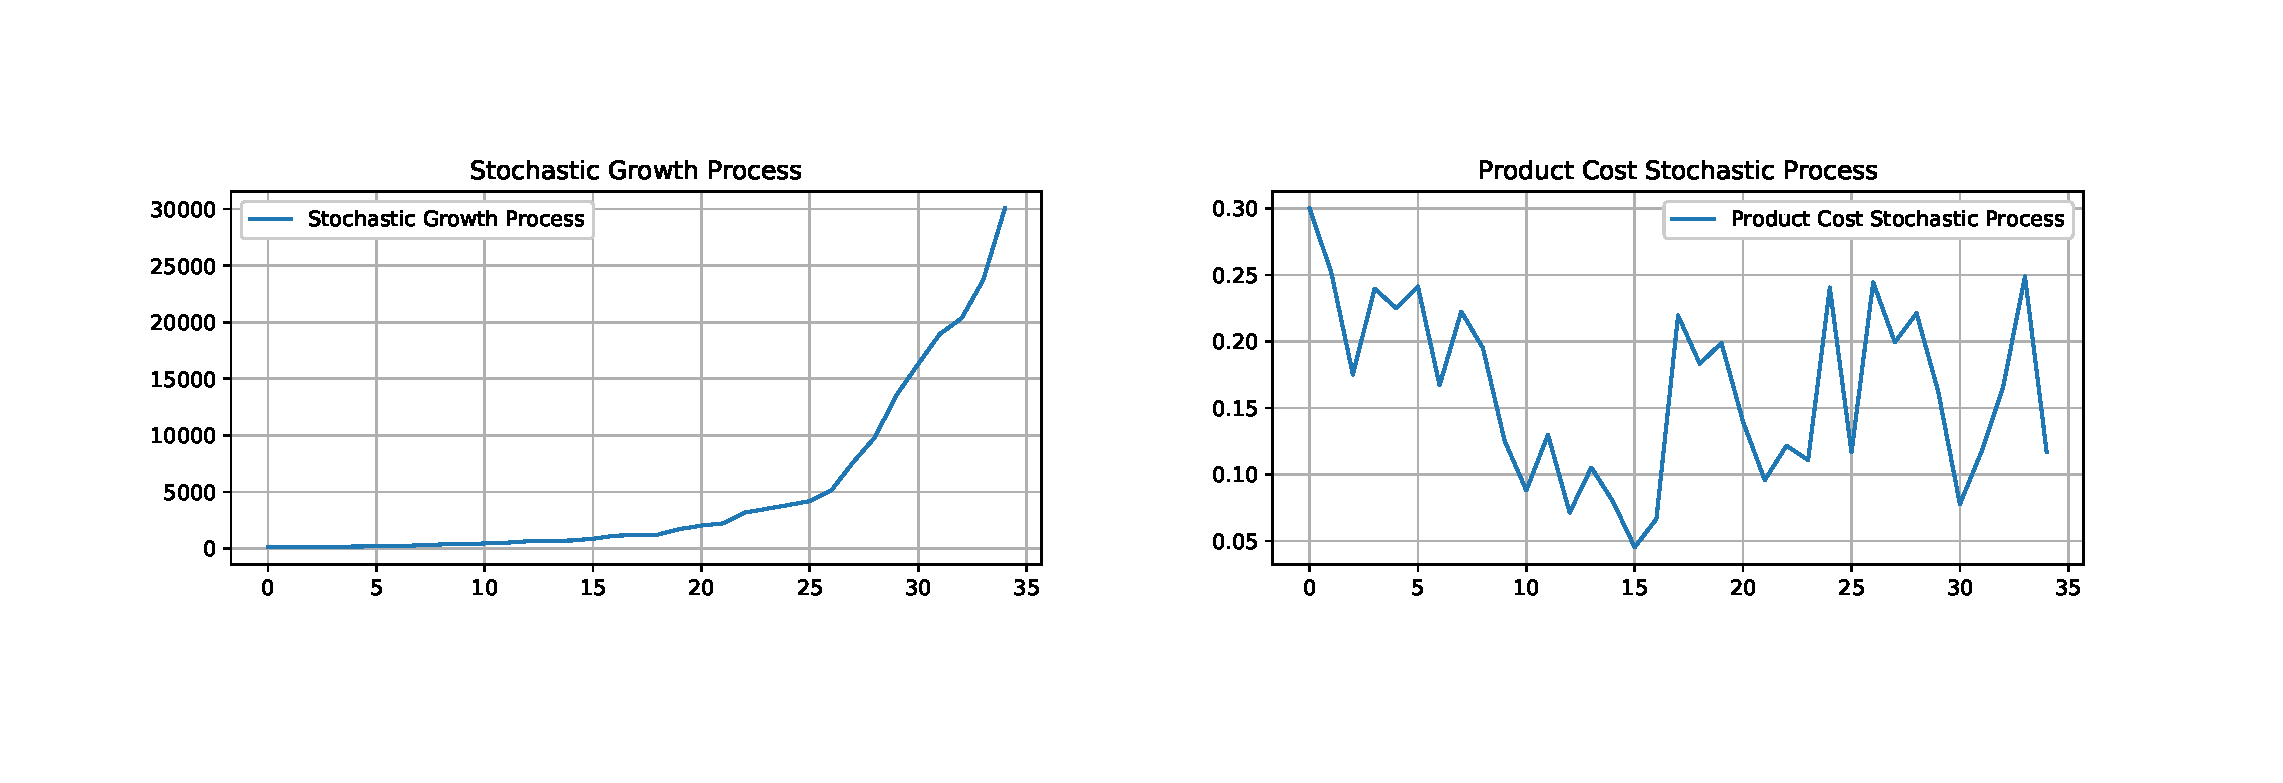
\includegraphics[width=1\textwidth]{images/components.eps}
    \caption{Components}
    \label{fig:components}
\end{figure}
\newpage


\section{cadCAD Simulation}
Once we finish defining the configuration file that contains the mathematical specifications and simulation commands, examples of which are shown in the previous section, we can then run simulations.  For our example here, we can look at the results at the beginning and the end of our model to see we started on 2018-01-01 and allowed our model to evolve every 30 days until 2020-12-26. We run our model 100 times, and take the mean of all of the simulations. As many of our components include random and varying factors, each simulation will run a little different from each other simulation. See the first five results at table \ref{table:FirstFive} and the last five at table \ref{table:LastFive}. \\ 


\begin{table}[h]
	\centering
	\begin{adjustbox}{max width=\textwidth}
	\begin{tabular}{lllllllllll}
		\toprule
		timestep & COGS             & R\&D & fiat\_reserve & overhead\_cost & product\_cost     & revenue   & seed\_money & tx\_volume \\
		0        & 0                & 0    & 0             & 100            & 0.3               & 0          & 0           & 100        \\
		1        & 6.34138          & 0    & 60068.01   & 100            & 0.24            & 108.01  & 100000      & 135.01   \\
		2        & 32.560         & 0    & 100139.18  & 100            & 0.20            & 171.18 & 100000      & 180.2203   \\
		3        & 38.09 & 0    & 100267.71  & 100            & 0.19 & 228.53  & 100000      & 240.61   \\
		4        & 48.75 & 0    & 100465.04  & 100            & 0.19            & 297.33  & 100000      & 311.50  
	\end{tabular}
\end{adjustbox}
\caption{First five time steps of the Monte Carlo Run}
\label{table:FirstFive}
\end{table}

\begin{table}[h]
	\centering
	\begin{adjustbox}{max width=\textwidth}
	\begin{tabular}{lllllllllll}
		\toprule
		timestep & COGS        & R\&D & fiat\_reserve & overhead\_cost & product\_cost & revenue          & seed\_money & tx\_volume       \\
		32       & 15103.09 & 1000 & 1029399.17 & 10100          & 0.17        & 90679.09 & 200000         & 91242.08 \\
		33       & 15701.94 & 1000 & 1112510.76 & 10100          & 0.19        & 93211.59 & 200000       & 93703.97 \\
		34       & 17344.59 & 2000 & 1197496.01 & 10100          & 0.177        & 95085.26 & 200000       & 95430.58 \\
		35       & 16565.27 & 2000 & 1284050.85 & 10100          & 0.1599        & 96654.83 & 200000       & 96960.90 \\
		36       & 15484.41 & 2000 & 1371673.12 & 10100          & 0.16        & 97722.27      & 200000       & 97912.61
	\end{tabular}
\end{adjustbox}
\caption{Last five time steps of the Monte Carlo Run}
\label{table:LastFive}
\end{table}
\noindent


We plotted the results of the simulation below in figure \ref{fig:results}. We can see that the Fiat Reserve stayed modest and mostly flat as the company was starting up, with the investor seed money keeping the company afloat. But as transactions and revenue began to expand, we can see tracked performance metrics began to increase. As the company begins, we can see a low value of overhead costs, but it slowly ramps up overtime as the company matures, rents office space, hires more employees, etc.  Cost of Goods Sold (COGS) starts off very low, but accelerates over time, as a result of the increased volume. Revenue is similar to COGS, but a smoother curve as the price of \$1 stays constant through the 36 month simulation. Transaction volume per month, as it is an exogenous (external to the system) process, it follows the same s-shaped curve we built as an individual component above. It is used to drive the rest of the model (the transaction volume can be modeled as well, but for this example we kept it simple.) We then look at the transaction Product Cost, which decreases after economies of scale are developed. Research and Development per month starts as zero and increases every 17 months by 1,000 per month. Finally, Gross Margin and EBITDA per month, show how we can layer on top of our modeling common business metrics. The sky is really the limit on what we can do with our simulations, as we can use existing design patterns we have internally developed, or build individual components from scratch to maximize accuracy for our clients. 

\begin{figure}[h]
	\centering
	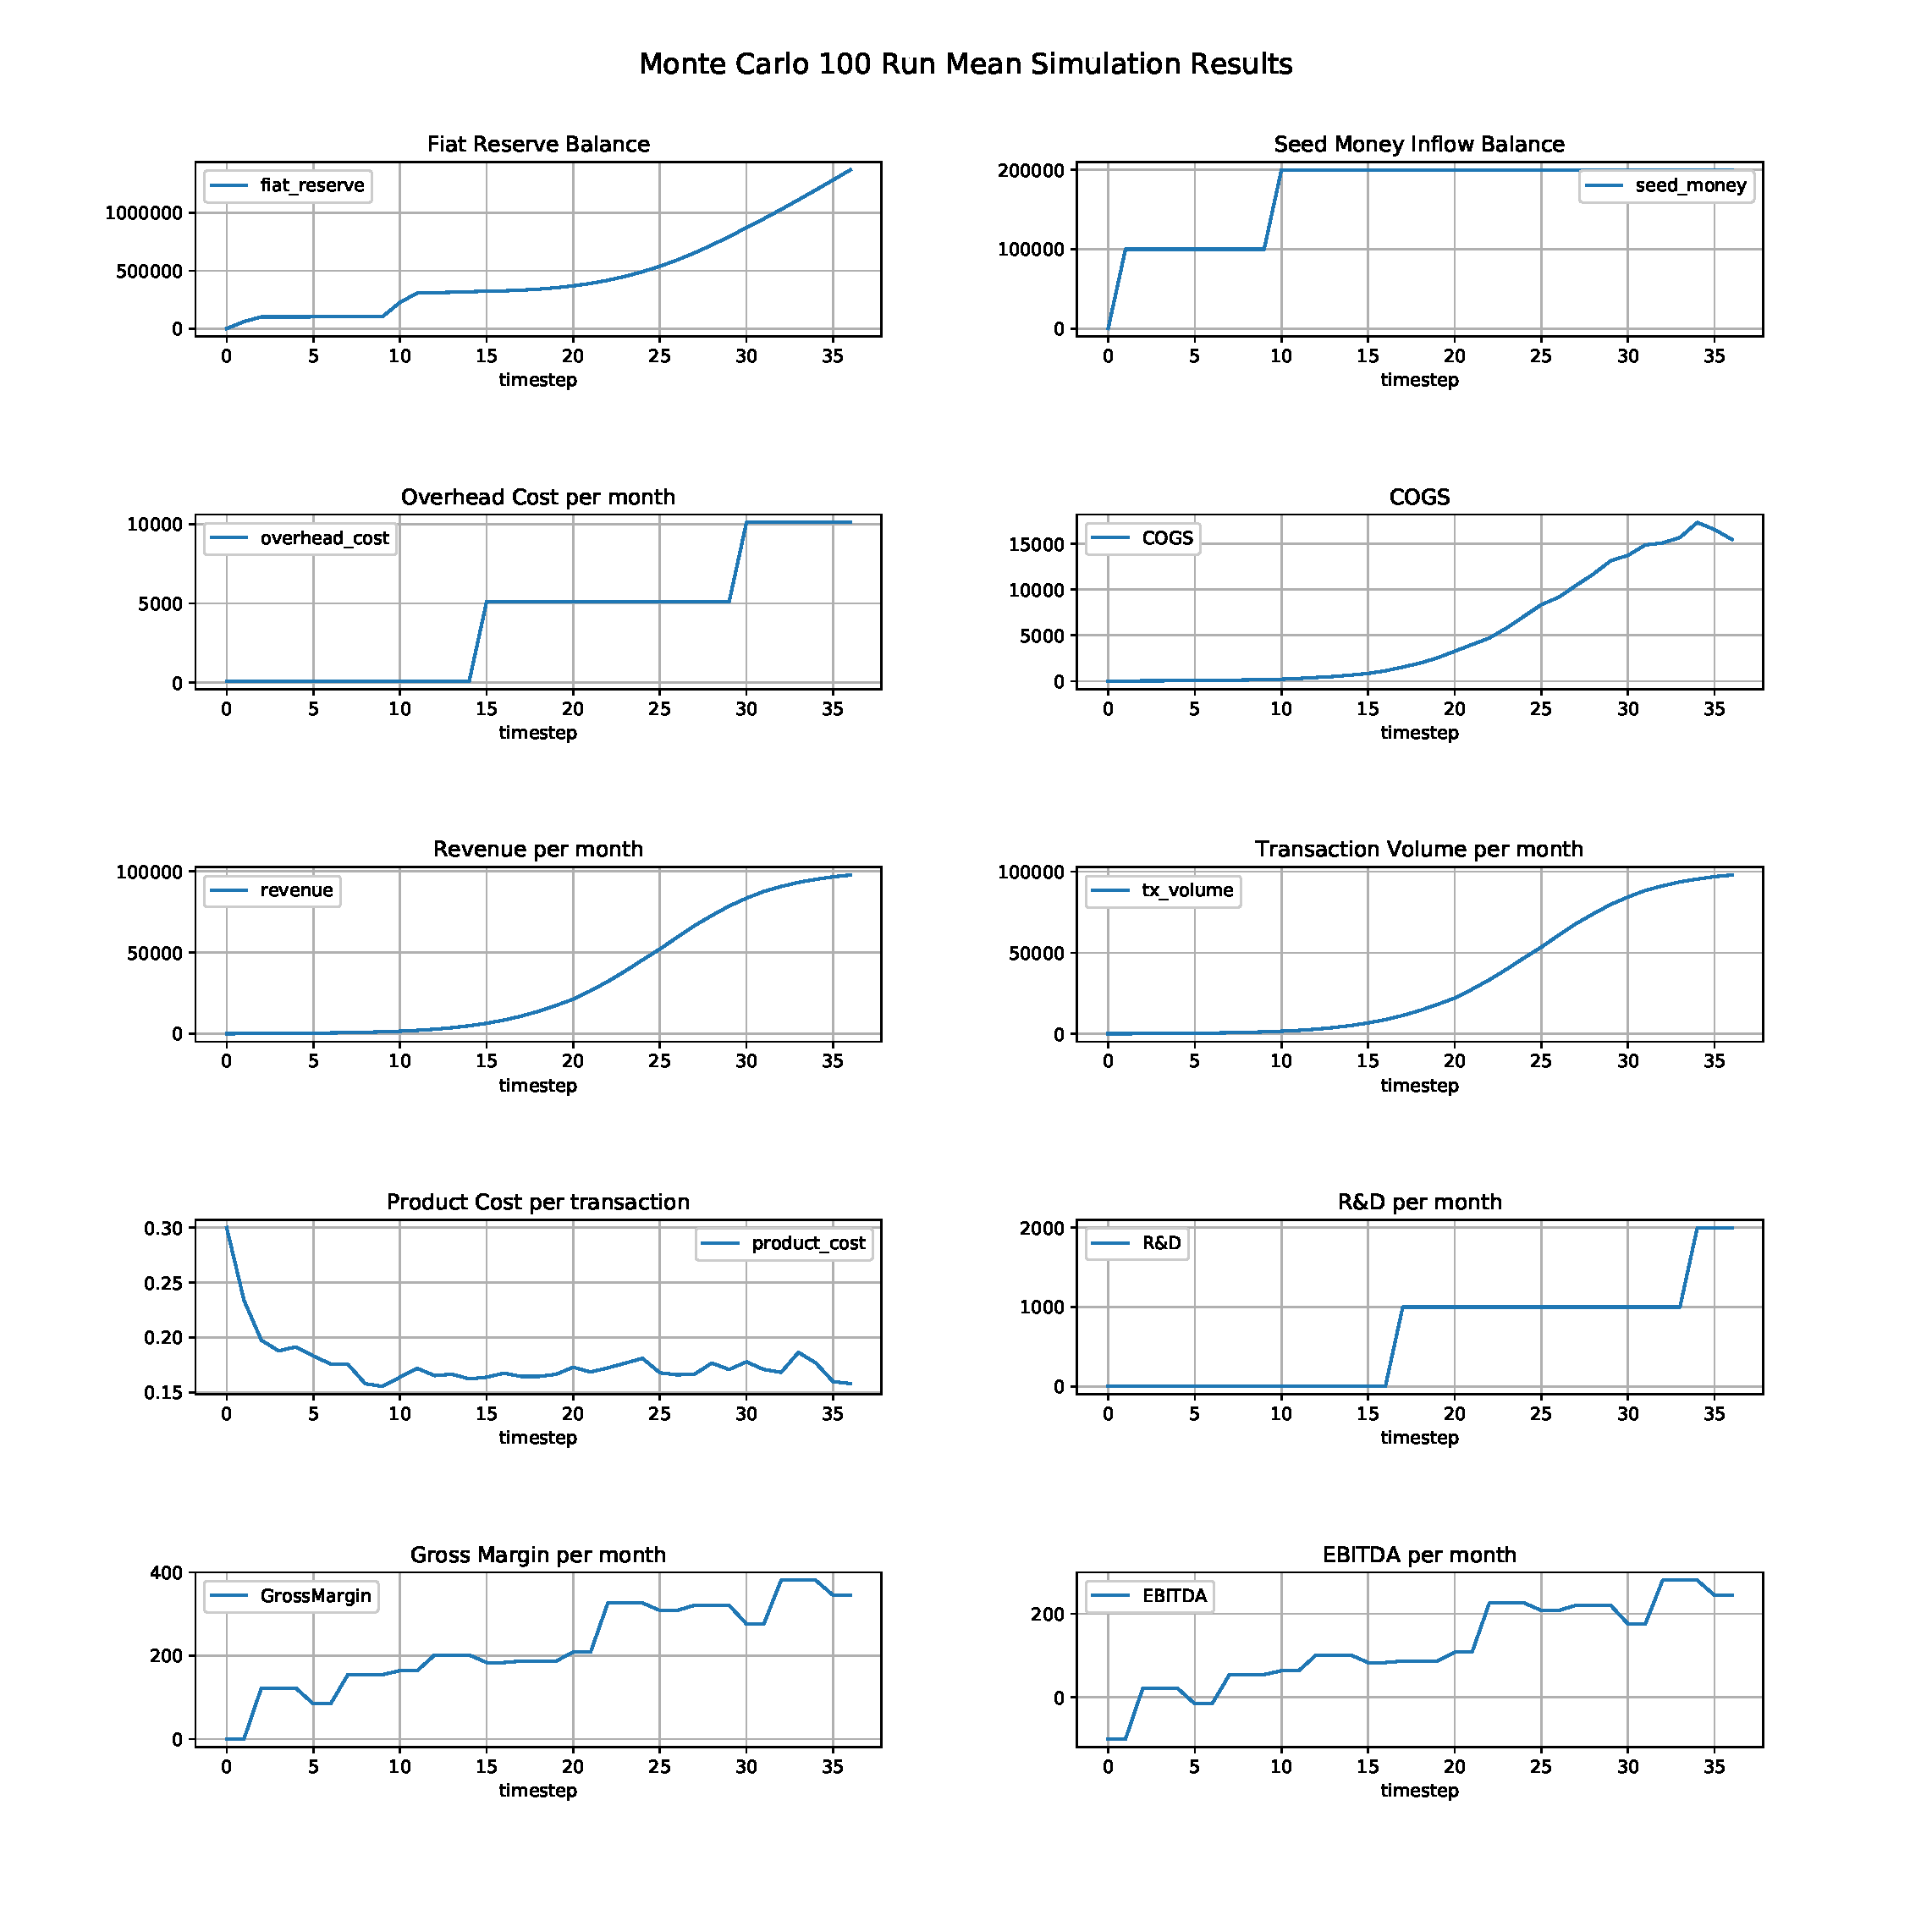
\includegraphics[width=1\textwidth]{images/Results.eps}
	\caption{Results}
	\label{fig:results}
\end{figure}

\section{Conclusion}
We have walked through a basic dynamical system ecosystem model taking in some external variables and seeing how the system responds to these signals and evolves. We observe that the policy and pricing incentives built into the model represent a successful business model. BlockScience goes in depth into each component, using cross functional teams of researchers to create novel solutions for our clients. What makes our modeling approach so powerful is that we can do A/B testing, or in other words, try slightly different policies and see how the system interacts and how the outputs we are concerned about respond. It is an extremely effective mechanism for making business decisions. Our methodologies, along with the cadCAD tool, enable us to help companies optimize their existing business models, mitigate risks, and help launch new companies or lines of business with the confidence of engineered and rigorously tested solutions.
\end{document}


